\documentclass[journal, a4paper]{IEEEtran}
\newcommand{\specialcell}[2][c]{%
  \begin{tabular}[#1]{@{}c@{}}#2\end{tabular}}
% some very useful LaTeX packages include:

%\usepackage{cite}      % Written by Donald Arseneau
                        % V1.6 and later of IEEEtran pre-defines the format
                        % of the cite.sty package \cite{} output to follow
                        % that of IEEE. Loading the cite package will
                        % result in citation numbers being automatically
                        % sorted and properly "ranged". i.e.,
                        % [1], [9], [2], [7], [5], [6]
                        % (without using cite.sty)
                        % will become:
                        % [1], [2], [5]--[7], [9] (using cite.sty)
                        % cite.sty's \cite will automatically add leading
                        % space, if needed. Use cite.sty's noadjust option
                        % (cite.sty V3.8 and later) if you want to turn this
                        % off. cite.sty is already installed on most LaTeX
                        % systems. The latest version can be obtained at:
                        % http://www.ctan.org/tex-archive/macros/latex/contrib/supported/cite/
                        
\usepackage{graphicx}
\usepackage{wrapfig}

\usepackage[T2A]{fontenc}			% кодировка
\usepackage[utf8]{inputenc}			% кодировка исходного текста
\usepackage[english,russian]{babel}	% локализация и переносы
\usepackage{graphicx}   % Written by David Carlisle and Sebastian Rahtz
                        % Required if you want graphics, photos, etc.
                        % graphicx.sty is already installed on most LaTeX
                        % systems. The latest version and documentation can
                        % be obtained at:
                        % http://www.ctan.org/tex-archive/macros/latex/required/graphics/
                        % Another good source of documentation is "Using
                        % Imported Graphics in LaTeX2e" by Keith Reckdahl
                        % which can be found as esplatex.ps and epslatex.pdf
                        % at: http://www.ctan.org/tex-archive/info/

%\usepackage{psfrag}    % Written by Craig Barratt, Michael C. Grant,
                        % and David Carlisle
                        % This package allows you to substitute LaTeX
                        % commands for text in imported EPS graphic files.
                        % In this way, LaTeX symbols can be placed into
                        % graphics that have been generated by other
                        % applications. You must use latex->dvips->ps2pdf
                        % workflow (not direct pdf output from pdflatex) if
                        % you wish to use this capability because it works
                        % via some PostScript tricks. Alternatively, the
                        % graphics could be processed as separate files via
                        % psfrag and dvips, then converted to PDF for
                        % inclusion in the main file which uses pdflatex.
                        % Docs are in "The PSfrag System" by Michael C. Grant
                        % and David Carlisle. There is also some information
                        % about using psfrag in "Using Imported Graphics in
                        % LaTeX2e" by Keith Reckdahl which documents the
                        % graphicx package (see above). The psfrag package
                        % and documentation can be obtained at:
                        % http://www.ctan.org/tex-archive/macros/latex/contrib/supported/psfrag/

%\usepackage{subfigure} % Written by Steven Douglas Cochran
                        % This package makes it easy to put subfigures
                        % in your figures. i.e., "figure 1a and 1b"
                        % Docs are in "Using Imported Graphics in LaTeX2e"
                        % by Keith Reckdahl which also documents the graphicx
                        % package (see above). subfigure.sty is already
                        % installed on most LaTeX systems. The latest version
                        % and documentation can be obtained at:
                        % http://www.ctan.org/tex-archive/macros/latex/contrib/supported/subfigure/

\usepackage{url}        % Written by Donald Arseneau
                        % Provides better support for handling and breaking
                        % URLs. url.sty is already installed on most LaTeX
                        % systems. The latest version can be obtained at:
                        % http://www.ctan.org/tex-archive/macros/latex/contrib/other/misc/
                        % Read the url.sty source comments for usage information.

%\usepackage{stfloats}  % Written by Sigitas Tolusis
                        % Gives LaTeX2e the ability to do double column
                        % floats at the bottom of the page as well as the top.
                        % (e.g., "\begin{figure*}[!b]" is not normally
                        % possible in LaTeX2e). This is an invasive package
                        % which rewrites many portions of the LaTeX2e output
                        % routines. It may not work with other packages that
                        % modify the LaTeX2e output routine and/or with other
                        % versions of LaTeX. The latest version and
                        % documentation can be obtained at:
                        % http://www.ctan.org/tex-archive/macros/latex/contrib/supported/sttools/
                        % Documentation is contained in the stfloats.sty
                        % comments as well as in the presfull.pdf file.
                        % Do not use the stfloats baselinefloat ability as
                        % IEEE does not allow \baselineskip to stretch.
                        % Authors submitting work to the IEEE should note
                        % that IEEE rarely uses double column equations and
                        % that authors should try to avoid such use.
                        % Do not be tempted to use the cuted.sty or
                        % midfloat.sty package (by the same author) as IEEE
                        % does not format its papers in such ways.

\usepackage{amsmath}    % From the American Mathematical Society
                        % A popular package that provides many helpful commands
                        % for dealing with mathematics. Note that the AMSmath
                        % package sets \interdisplaylinepenalty to 10000 thus
                        % preventing page breaks from occurring within multiline
                        % equations. Use:
%\interdisplaylinepenalty=2500
                        % after loading amsmath to restore such page breaks
                        % as IEEEtran.cls normally does. amsmath.sty is already
                        % installed on most LaTeX systems. The latest version
                        % and documentation can be obtained at:
                        % http://www.ctan.org/tex-archive/macros/latex/required/amslatex/math/



% Other popular packages for formatting tables and equations include:

%\usepackage{array}
% Frank Mittelbach's and David Carlisle's array.sty which improves the
% LaTeX2e array and tabular environments to provide better appearances and
% additional user controls. array.sty is already installed on most systems.
% The latest version and documentation can be obtained at:
% http://www.ctan.org/tex-archive/macros/latex/required/tools/

% V1.6 of IEEEtran contains the IEEEeqnarray family of commands that can
% be used to generate multiline equations as well as matrices, tables, etc.

% Also of notable interest:
% Scott Pakin's eqparbox package for creating (automatically sized) equal
% width boxes. Available:
% http://www.ctan.org/tex-archive/macros/latex/contrib/supported/eqparbox/

% *** Do not adjust lengths that control margins, column widths, etc. ***
% *** Do not use packages that alter fonts (such as pslatex).         ***
% There should be no need to do such things with IEEEtran.cls V1.6 and later.
\usepackage{soul}
\usepackage{soulutf8}

\usepackage{ amssymb }
% Your document starts here!
\begin{document}

% Define document title and author
	\title{{\large Лабораторная работа № 4.7.1}\\Двойное лучепреломление
}
	\author{Ступаков Олег \hspace{11.62cm} 1 марта 2019 г. \\ 722 группа 
	\hspace{11.71cm} ~г. Долгопрудный~
	\thanks{}}
	\markboth{{\small К}афедра общей физики {\small МФТИ }}{}
	\maketitle

% Write abstract here
%\begin{abstract}

%\end{abstract}

% Each section begins with a \section{title} command
\section*{}
	% \PARstart{}{} creates a tall first letter for this first paragraph
	\PARstart{}{~Ц{\small ель работы}}{\large :} изучение зависимости показателя преломления
необыкновенной волны от направления в двоякопреломляющем кристалле; определение главных показателей преломления $n_o$--обыкновенной и $n_{e}$--необыкновенной волны в кристалле; наблюдение эффекта полного внутреннего отражения.\vspace{0.15cm}
	\PARstart{}{{\footnotesize ~}O{\small борудование}}{\large :}~гелий-неоновый лазер, вращающийся столик с неподвижным лимбом, призма из исландского шпата, поляроид
% Main Part
\section{Теоретическое введение}
 Для
характеристики оптических свойств анизотропной среды требуетс
я девять величин $\varepsilon_{ij}$ , образующих тензор диэлектрической проницаемости. Он вводитс
я посредством соотношений
	\begin{equation}\label{}
	D_i =\sum_{j}\varepsilon_{ij}E_j ~~~~(i,j= x,y,z). 
	\end{equation}
	
	Поворотом системы координат тензор диэлектрической проницаемости приводится к диагональному виду, и проекции векторов
 $\vec D\quad $и
$\vec E\quad$ на оси
координат связаны
простыми соотношениями:
\[D_x = \varepsilon_xE_x,~~ D_y = \varepsilon_yE_y,~~ D_z = \varepsilon_zE_z.\]

В оптически одноосном кристалле,
каковым является исландский
шпат, $\varepsilon_x=\varepsilon_y=\varepsilon_{\perp}$ и
$\varepsilon_z=\varepsilon_{\|}$. В дальнейшем нам потребуетс
я связь между проекциями
векторов
$\vec D$ и
$\vec E$ на оптическую ось кристалла $(\vec D_{\|}~\text{и}~\vec E_{\|})$	 и на плоскость,
перпендикулярную оси $(\vec D_{\perp}~\text{и}~\vec E_{\perp})$	
\begin{equation}\label{}
\overrightarrow{D}_{\|}=\varepsilon_{\|}\overrightarrow{E}_{\|}~~
\text{и} ~~
 \overrightarrow {D}_{\perp}= \varepsilon_{\perp}\overrightarrow{E}_{\perp}
\end{equation}
\begin{wrapfigure}{l}{3.3cm}
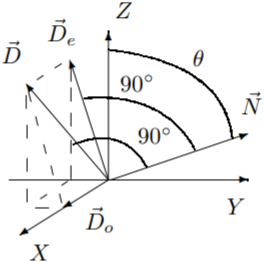
\includegraphics[width=3.5cm]{fig1}
\caption{Расположение векторов~$\vec{N}$~и~$\vec{D}$  в анизотропной среде.}
\end{wrapfigure}Волну, распространяющуюся
в одноосном кристалле, можно разделить на две линейно
поляризованные волны: обыкновенную, вектор электрической
индукции
$\vec{D}_o$ которой перпендикулярен главному сечению,
и необыкновенную, с вектором
электрической индукции
$\vec{D}_e$, лежащим в главном сечении (рис. 1).
\textit{Главным сечение
м кристалла}
называется плоскость, в которой
лежит оптическая ось кристалла
и нормаль
к фронту волны.
Рассмотрим вначале обыкновенную волну, в которой вектор
$\vec{D}_o$ перпендикулярен главному сечению.
Тогда
$D_{oz}
= 0$, и из
условия
$Dz = \varepsilon_zE_z$ следует, что
$E_{oz}
= 0.$ Кроме того, так как
$D_{oy}
= \varepsilon_\perp
E_{oy}$
и
$D_{ox}
= \varepsilon_\perp$
Eox, то можно записать
\begin{equation}
\vec D_{o}
= \varepsilon_\perp \vec{E}_o
\end{equation}Введем единичный вектор нормали
$\vec{N}$ к фронту волны
и скорость распространения фронт
а в направлении этой нормали $v$. Тогда, в соответсвии со следствиями  уравнений Максвелла 
\begin{equation}
\vec{D}=-\frac{c}{b}\left[\vec{N}\vec{H}\right];~~
\vec{B}=\frac{c}{v}\left[\vec{N}\vec{E}\right].
\end{equation}
Из (3) и (4) имеем
\[
\begin{aligned}
D_o = \frac{c}{v_o}H_o&,~~~ H_o=\frac{c}{v_o}E_o ,~~~
\varepsilon_\perp E_o=\frac{c}{v_o}H_o\\
v_o=&\frac{c}{\sqrt{\varepsilon_{\perp}}} ~~~\text{и}~~~ n_o = \frac{c}{v_o}=\sqrt{\varepsilon_{\perp}}
\end{aligned}
\]
Таким образом, скорость распространения обыкновенной волны
и ее показатель преломления не зависят от направления распространения.
У необыкновенной волны вектор
$\vec{D}_e$ не параллелен
$\vec{E}_e$, и связь между
ними сложнее, чем в (2).
Для того чтобы найти скорость распространения $v$ и показатель преломления необыкновенной волны
$n=c/v$, достаточно найти связь между вектором электрической индукции этой волны
$\vec{D}_e$ и проекцией на него
вектора электрического поля волны
$E_{eD}$. Тогда, подставляя
$De = \varepsilon E_{eD}$
в (4), приходим
к соотношениям\[
\varepsilon E_{eD} = \frac{c}{v}H_e;~~~
H_e=\frac{c}{v}E_{eD},
\]
формально тождественным с соотношениями для обыкновенной волны.
Роль величины $\varepsilon_{\perp}$ теперь играет величина $\varepsilon$, а показатель преломления
необыкновенной волны равен
$\sqrt{\varepsilon}$.

Найдем связь между
${D}_e$ и
$E_{eD}$. Для этого разложим векторы
$\vec{D}_e$ и $\vec{E}_e$ на составляющие, параллельные
и перпендикулярные оси кристалла:
\[
\begin{aligned}
\vec{D}_e&=\vec{D}_{e\|}+\vec{D}_{e\perp}.\\
\vec{E}_e&=\vec{E}_{e\|}+\vec{E}_{e\perp}.
\end{aligned}
\]
Учитывая (2), находим
\[
E_{eD}=\frac{\vec{E}_e\vec{D}_e}{D_e}=
\frac{E_{e\|}D_{e\|}+E_{e\perp}D_{e\perp}}{D_e}=\frac{D_{e\|}^2/\varepsilon_{\|}+D_{e\perp}^2/\varepsilon_{\perp}}{D_e}
\]
или
\[
E_{eD}=D_e\left(\frac{\sin^2{\theta}}{\varepsilon_{\|}}+\frac{\cos^2{\theta}}{\varepsilon_{\perp}}\right)=\frac{D_e}{\varepsilon},
\]
где $\theta$-- угол между оптической осью
$Z$ и волновой нормалью $N$ (рис. 1):
\begin{equation}
\sin{\theta}=\frac{D_{e\|}}{D_e},~~\cos{\theta}=\frac{D_{e\perp}}{D_e}
\end{equation}

Таким образом, $\varepsilon$ и соответственно скорость распространения
и показатель преломления необыкновенной волны зависят от угла между оптической осью кристалла
и направлением распространения волны.

Выпишем выражение для показателя преломления необыкновенной
волны
$n=\sqrt{\varepsilon}$ через главные показатели преломления
$n_o, n_e$ и угол $\theta$:
\begin{equation}
\frac{1}{\left[n(\theta)\right]^2}=
\frac{\sin^2{\theta}}{n_e^2}+
\frac{\cos^2{\theta}}{n_o^2}
\end{equation}
При $n_o - n_e \ll n_o$ и
$n_e$ (для исландского шпат
а
$no = 1,655, ne = 1,485$
для $\lambda= 0,63~\text{мкм}$) (6) можно упростить:
\begin{equation}
n(\theta)\approx n_e + (n_0-n_e)\cos^2{\theta}.
\end{equation}
Рассмотрим,
как по преломлению лучей в кристаллической призме можно
определить показатели преломления для обыкновенной
и необыкновенной волны.
В работе исследуетс
я одна из двух призм, составляющих
поляризатор (рис. 2).
\begin{figure}[h!]
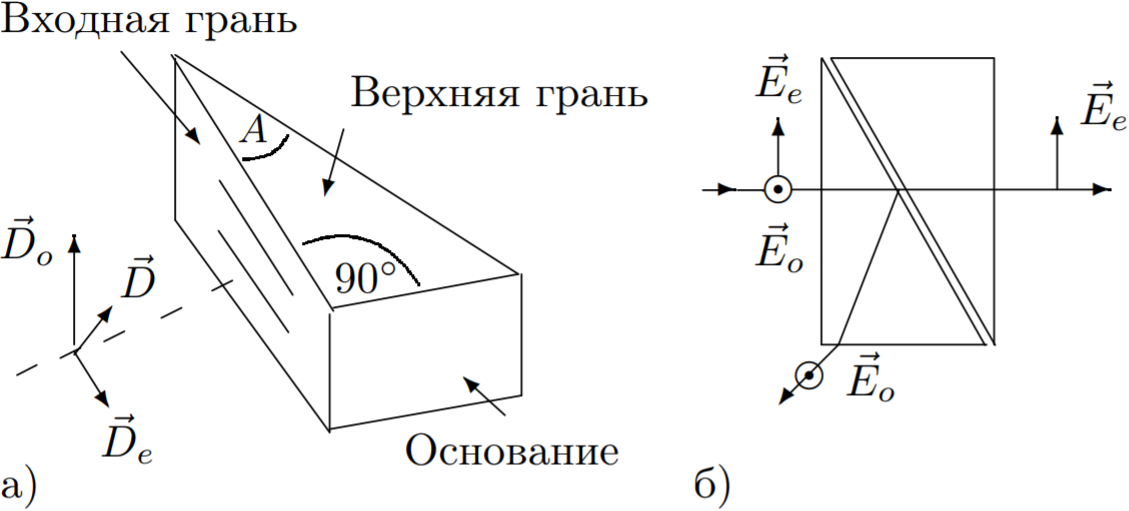
\includegraphics[scale=0.36]{fig2}
\caption{а) Исследуемая призма из исландского шпата.
Штриховкой указано направление оптической оси кристалла. б) Хо
д лучей в поляризационной призме
}
\end{figure}
Для обыкновенной волны
$n$ не будет зависеть от угла $\theta$. Для неё из закона Снеллиуса в соответсвии с рис. 3 
\[
\sin\varphi_1=n\sin\beta_1;
\]
\[\sin\varphi_2=n\sin\beta_2=n\sin{(A-\beta_1)}.\]
Откуда 
\begin{equation}
n=\frac{q}{\sin A}\sqrt{\sin^2\varphi_1 + \sin^2{\varphi_2}+2\sin{\varphi_1}\sin{\varphi_2}\cos{A}}
\end{equation}
\begin{wrapfigure}{r}{3.9cm}
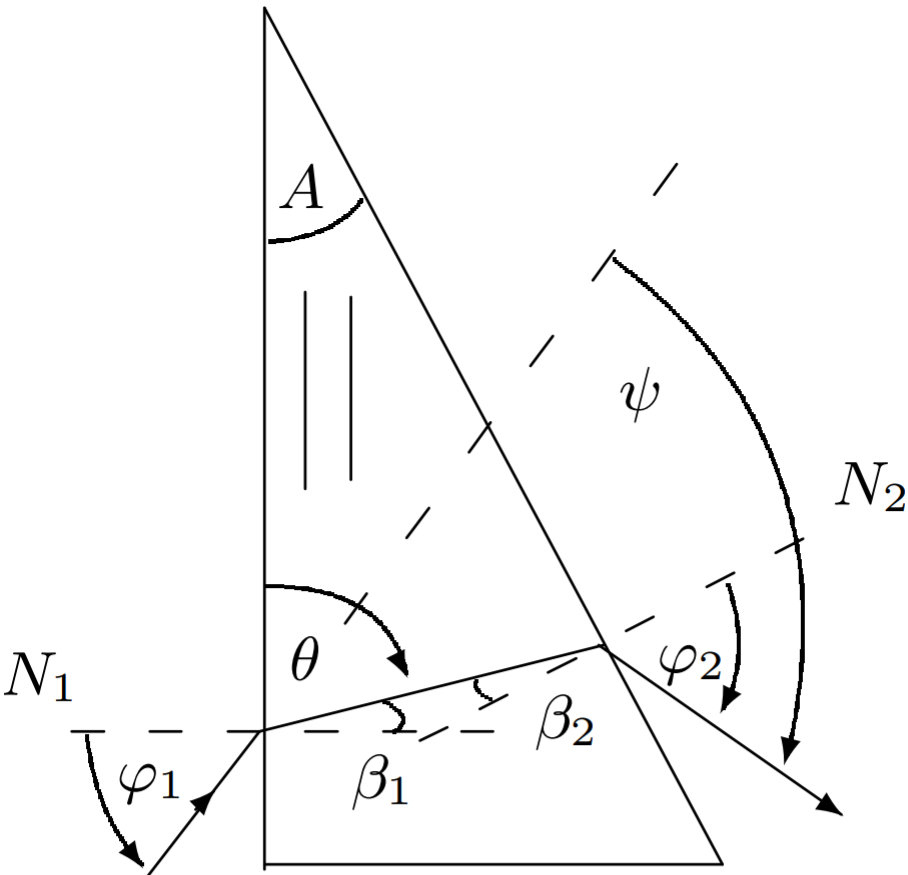
\includegraphics[width=4.3cm]{fig3}
\caption{Ход лучей в призме.}
\end{wrapfigure}

Для необыкновенной волны зависимость
n от $\theta$ должна описыватьс
я выражением (6).

Показатель преломления призмы из изотропного материала
удобно
находить по углу наименьшего отклонения луча от первоначального направления. Угол отклонения луча призмой ($\psi$ на рис. 3) минимален для
симметричного
хода лучей, т.е.
когда
$\varphi_1=\varphi_2$ Тогда показатель преломления можно рассчитать по формуле
\begin{equation}
n=\frac{\sin{(\frac{\psi_m+A}{2})}}{\sin{(\frac{A}{2})}},
\end{equation}
где
$\psi_m$-- угол наименьшего отклонения.
\section{Экспериментальная установка}
\begin{figure}[h!]
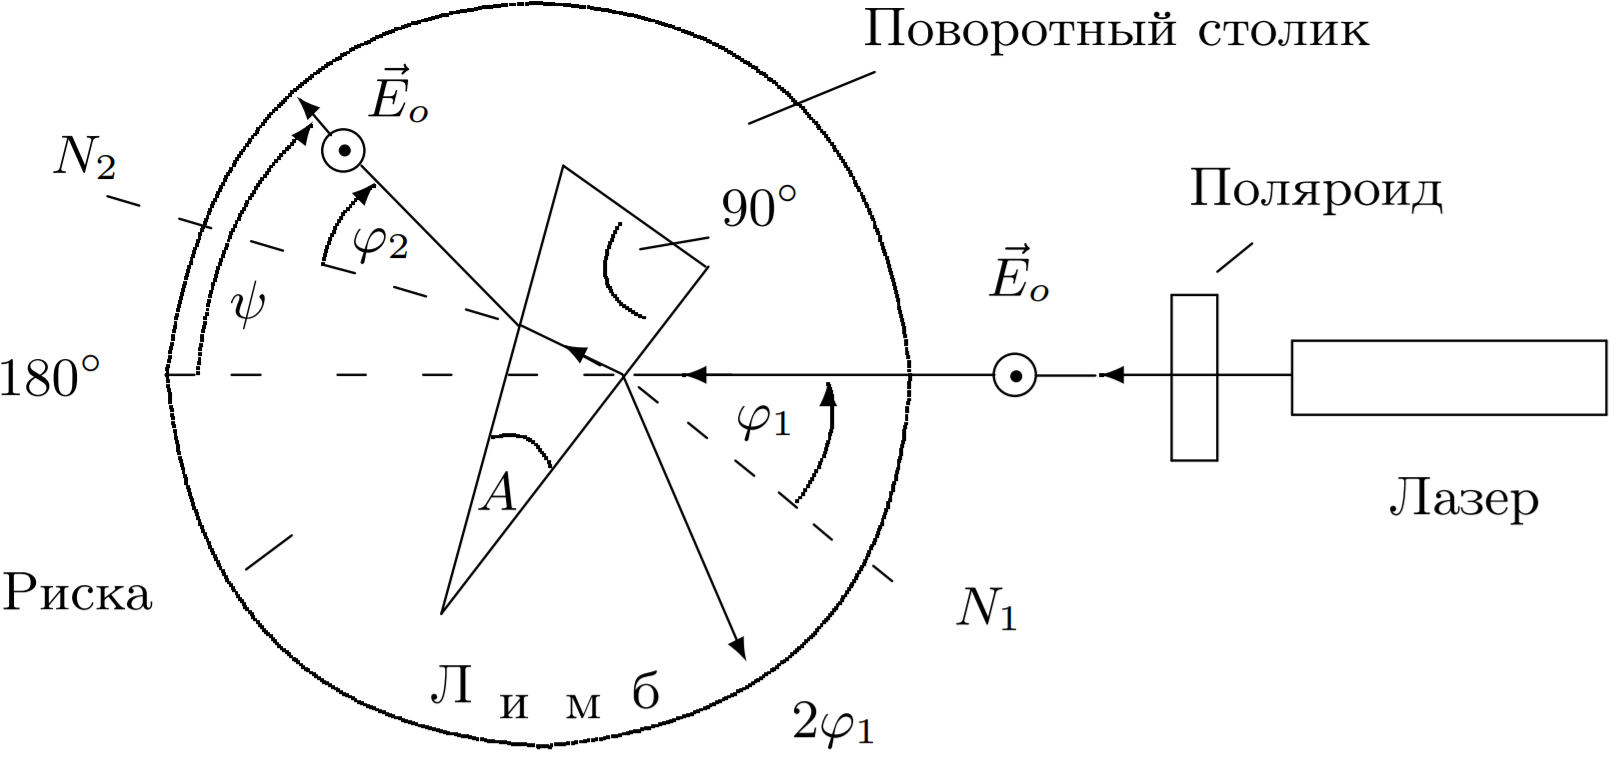
\includegraphics[scale=0.26]{fig4}
\caption{Схема экспериментальной установки
}
\end{figure}
Схема экспериментальной
установки изображена на рис. 4. Источником излучения служит Не-Nе лазер
($\lambda
= 0,63 \text{мкм}$). Излучение лазера поляризовано линейно за счет наличия брюстеровских окошек в кювете лазера. Направление вектора
$\vec{E}$ в
луче можно изменять с помощью поляроида,
установленного на выходе
лазера. Исследуемая призма из исландского шпата закреплена в центре
поворотного столика с неподвижным лимбом для отсчета углов.

Преломляющий угол A призмы (рис. 3) можно рассчитать, если известны угловые
координаты нормалей
$N_1$ и
$N_2$ к преломляющим (рабочим) граням призмы, прилежащим преломляющему углу. Грань, противолежащая преломляющему углу, называется основанием призмы.
Штриховкой указано направление оптической оси.

Обычно
ход лучей в призме таков, что
и падающий,
и преломлённый
лучи отклоняются от нормалей в сторону основания призмы, при этом
углы
$\varphi_1$ и
$\varphi_2$ считаются положительными.

Угол падения
$\varphi_1$ определяется по поло
жению луча, отражённого от
передней (входной) грани призмы (рис.~4). Из рис. 3 можно получить
связь углов
$\varphi_1$ и
$\varphi_2$:
\begin{equation}
\varphi_2=A+\psi-\varphi_1
\end{equation}
а угол $\psi$-- отклонение преломлённого луча от первоначального направления-- определяется по разности отсчётов на лимбе между точками,
куда попадает луч в отсутствие призмы,
и точкой, куда попадает преломлённый луч.

При монотонном увеличении угла падения угол
$\psi$ сначала уменьшается,
а затем снова начинает увеличиваться. Минимальное отклонение
соответствует симметричному
ходу луча: внутри призмы луч идёт перпендикулярно биссектрисе угла
A, а
$\varphi_1$ =
$\varphi_2$. Углы наименьшего отклонения
$\psi_m$
m различны для обыкновенного
и необыкновенного лучей.

Угол
A подобран так, что призма мо
жет выполнять роль поляризатора: при нормальном падении луча на первую преломляющую грань
из призмы выходит только один луч,
а другой испытывает полное внутреннее отражение на второй грани. При повороте призмы на небольшой угол на экране появляютс
я оба преломлённых луча. Можно подобрать такой угол падения, при
котором исчезнет второй преломлённый
луч. Область углов поворот
а призмы, в которой обеспечиваетс
я пространственное разделение лучей с взаимно ортогональной поляризацией, определяетс
я относительной разницей главных показателей преломления
$n_o$ и
$n_e$.
\section{Ход работы}
{\normalsize 1.}{\normalsize Определим угол $A$ при вершине призмы.}
Сначал добьёмся, чтобы луч, отражённый от входной грани (длинного
катета), шёл
точно назад,  заметим положение отсчётной риски на лимбе($\varphi_K$),
а затем повторим эту операцию для второй рабочей грани (гипотенузы, $\varphi_G$). По разнице этих двух отсчётов найдём угол A.
\begin{table}[h!]
\begin{center}
\begin{tabular}{|c|c|c|}
\hline 
$\varphi_K$ & $\varphi_G$ & A \\ 
\hline 
$251^{\circ}$ & $108^{\circ}$& $(37\pm1)^{\circ}$\\ 
\hline 
\end{tabular}
\end{center}
\caption{Определение угла А} 
\end{table}

 Вращая столик с призмой, снимем зависимость углов отклонения на
выходе из призмы для обыкновенной
и необыкновенной волн от угла
падения луча на призму;
будем замерять координату $2\varphi_1$ луча, отраженного от входной грани призмы — длинного катета, и координаты
каждого из преломлённых лучей.

Проведём серию измерений, меняя $\varphi_1$ в диапазоне $10$-$70^{\circ}$ через $5^{\circ}$, а вблизи минимального угла $\psi_m$-- через $2,5^{\circ}$.  Проведём расчет на компьютере с помощью программы SIGMA PLOT и запишем рассчитанные значения $\cos^2{\theta}, n_o(\theta)~ \text{и}~ n_e(\theta)$ и окончательные результат -- $n_o ~\text{и}~ n_e$.

\begin{table}[h!]
\begin{center}
\begin{tabular}{|c|c|c|c|c|c|c|c|}
\hline 
$N_{\text{т}}$ & $\psi_1$ & $\psi_o$ & $\psi_e$ & $\cos^2{\theta_o}$ & $\cos^2{\theta_o}$ & $n_o$ & $n_e$ \\ 
\hline 
1 & 10 & 31,5 & 22 & 0,01 & 0,01 & 1,649 & 1,489 \\ 
\hline 
2 & 15 & 29 & 21 & 0,02 & 0,03 & 1,648 & 1,494 \\ 
\hline 
3 & 17,5 & 28,5 & 20,5 & 0,03 & 0,04 & 1,654 & 1,493 \\ 
\hline 
4 & 20 & 27,5 & 20 & 0,04 & 0,05 & 1,648 & 1,489 \\ 
\hline 
5 & 22,5 & 27 & 20 & 0,05 & 0,07 & 1,647 & 1,494 \\ 
\hline 
6 & 25 & 27 & 20 & 0,07 & 0,08 & 1,655 & 1,497 \\ 
\hline 
7 & 27,5 & 26,5 & 20 & 0,08 & 0,09 & 1,649 & 1,499 \\ 
\hline 
8 & 30 & 26,5 & 20 & 0,09 & 0,11 & 1,652 & 1,499 \\ 
\hline 
9 & 32,5 & 26,5 & 20,3 & 0,11 & 0,13 & 1,652 & 1,505 \\ 
\hline 
10 & 35 & 26,4 & 20,5 & 0,12 & 0,15 & 1,648 & 1,506 \\ 
\hline 
11 & 375 & 26,5 & 21 & 0,14 & 0,16 & 1,647 & 1,513 \\ 
\hline 
12 & 40 & 27 & 21 & 0,15 & 0,18 & 1,653 & 1,506 \\ 
\hline 
13 & 42,5 & 27,2 & 21,5 & 0,17 & 0,2 & 1,65 & 1,51 \\ 
\hline 
14 & 45 & 27,8 & 22 & 0,18 & 0,22 & 1,654 & 1,511 \\ 
\hline 
15 & 50 & 29 & 23,5 & 0,21 & 0,25 & 1,657 & 1,522 \\ 
\hline 
16 & 55 & 30 & 25,5 & 0,25 & 0,28 & 1,645 & 1,536 \\ 
\hline 
17 & 60 & 32 & 27 & 0,28 & 0,32 & 1,649 & 1,529 \\ 
\hline 
18 & 65 & 34,5 & 29,5 & 0,3 & 0,35 & 1,655 & 1,537 \\ 
\hline 
19 & 70& 37 & 32,5 & 0,32 & 0,37 & 1,651 & 1,546 \\ 
\hline 
\end{tabular}
\end{center} 
\caption{Таблица зависимости $n_o$ и $n_e$ от $\theta$}
\end{table}
По полученным~данным построим~на одном графике зависимости $n_o(\cos\theta) ~\text{и}~ n_e(\cos\theta)$ и определим главные показатели преломления $n_o$ и $n_e$ 


\begin{figure}[h!]
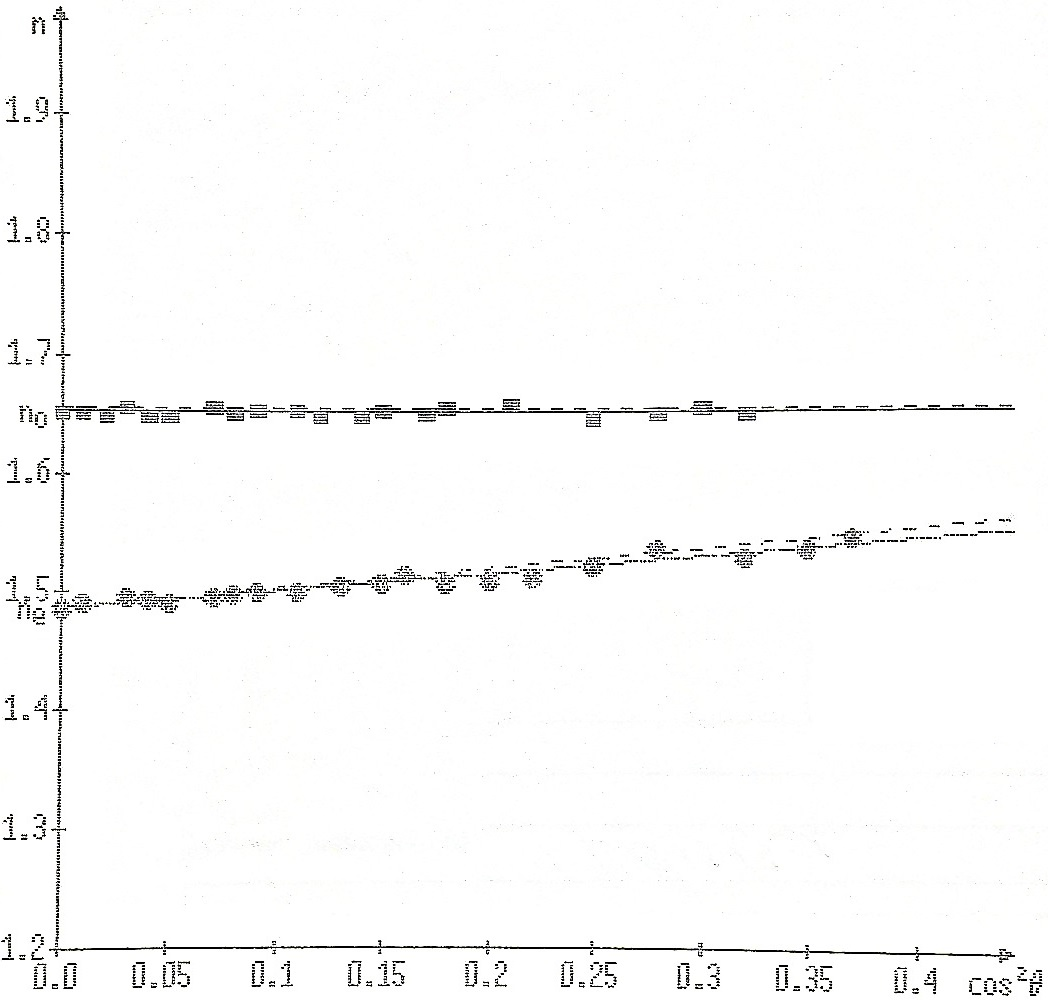
\includegraphics[width=9cm]{fig5}
\caption{График зависимости $n_o$ и $n_e$ от $\cos\theta$}
\end{figure}
Полученные значения $n_o$ и $n_e$ :

\fbox{$n_o=1,652\pm0,003$}

 \fbox{$n_e=1,486\pm0,004$} \\[1pt]

Как видими, результаты неплохо согласуются с табличными данными ($n_{o_\text{табл}}=1,655$, $n_{e_\text{табл}}=1,485$)

Из основной серии измерений определим средние значения углов наименьшего отклонения $\psi_m$; по формуле (9) рассчитаем показатели преломления $n_o$ и $n_e$:
\[
\begin{aligned}
\psi_{mo}= 26,4^{\circ}& ~~~ n_{o\psi} = 1,65 \\
\psi_{me}= 20,0^{\circ}& ~~~ n_{e\psi} = 1,5
\end{aligned}
\]

Для определения углов падения, соответствующих полному внутреннему отражению, сначала установим призму так, чтобы были видны оба
преломлённых луча; затем, уменьшая угол падения, добьёмся для каждого из лучей выполнения условий полного отражения от второй грани
призмы ($\varphi_2=90^{\circ}$); определите соответствующие углы $\varphi_{1e}$ и $\varphi_{1o}$ с учётом
знака.
Рассчитаем значения $n_o$ и $n_e$ по формуле (8):
\[
n_{o\varphi}=1,660\pm0,013 ~~~~ n_{e\varphi}= 1,49 \pm 0,015
\]
\section{Вывод}
В результате проведенной работы мы определили главные показатели преломления исландского шпата тремя способами: сняв зависимость
$\psi = f(\varphi_1)$ для обыкновенной
и
необыкновенной волны; определив углы наименьшего отклонения
$\psi_m$для обыкновенной
и необыкновенной волны; измерив для
каждого из
лучей угол падения
$\varphi_1$ в условиях полного внутреннего отражения. Наилучшие точность и приближенность к табличным значениям соответствуют первому способу.
\end{document}
